\documentclass{ctexart}
\usepackage{graphicx,picinpar}
\usepackage{float}
\usepackage{geometry}
\geometry{a4paper,scale=0.7}
\title{Homework 12: 房价预测模型}
\author{康子熙}
\date{\today}
\begin{document}
\maketitle

\section{摘要}
在这次房价预测模型的作业中,我依据homework11的提示,同时结合了一些自己对模型的理解,成功完成了任务,
构建出了一个\textbf{MAPE误差小于0.3100}的模型,达到了预测模型指标\textbf{2分}的要求。\par
在这次实验报告中,我将向老师和助教学长详细的说明模型构建的背景,数据探索性的分析,特征工程的处理过程以及模型的建立,
并且进行分析和总结。\par
下面,我先将我的模型的结果展示出来,以便老师和助教学长查看:
\begin{figure}[H]
    \centering
    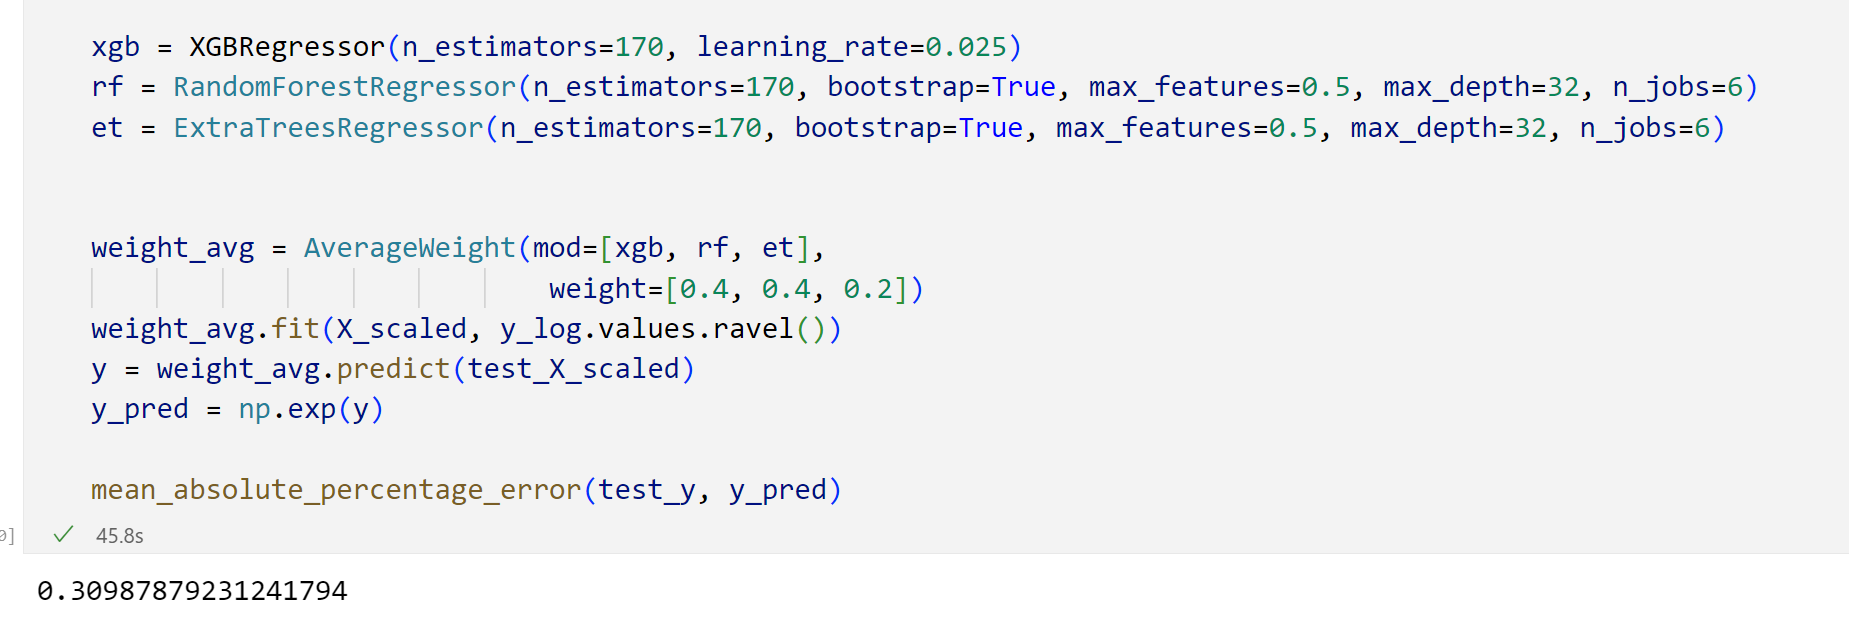
\includegraphics[scale=0.5]{./output.png}
    \caption{模型结果}
    \label{figure}
\end{figure}
\par

\section{模型构建背景}
由于homework12的任务是基于homework11代码的引导进行的,所以在构建homework12的预测模型时,我先对homework11的模型制作过程进行了总结,
以便于我更好的构建homework12的模型。\par
homework11在搭建预测模型时一共做了如下几个步骤:
\begin{enumerate}
    \item 数据可视化:可视化数据以清晰的理解各个数据的相关程度以及是否有异常值
    \item 数据处理:删除异常值,对缺失值进行填充
    \item 特征工程:将类别特征转化为数值特征,并且建立管道以试验不同的功能组合及添加特征
    \item 特征工程-特征选择:使用Lasso回归选择特征,观察每个特征的重要性
    \item 模型建立:使用5折交叉验证验证模型的最优参数,并且对模型进行集成训练
    \item 模型建立Plus:使用stacking将原始特征和堆叠生成的特征结合,构建新的模型
    \item 模型预测:运行模型,观察输出结果,如若不理想则修改模型参数或结果并重新训练
\end{enumerate}
\par
在这次的作业中,我将按照homework11的步骤,对homework12的模型进行构建。但是homework12较homework11,在data上有一些显著的区别,所以
不能完全仿照homework11进行构建,事实上,全部模仿homework11的模型,运行时MAPE会在0.33附近,远远达不到0.31的要求,
所以我在构建模型时还选择了一些其它的方法,以便于提高模型的准确度。\par
下面,我将对homework12的模型构建过程进行详细的说明。

\section{数据探索性分析}
根据作业中提供的数据字典,我了解了各个数据的用途,发现数据有很多缺失值,于是我进行了数据的删除、缺省数据的补充等操作。
\par
    \subsection{数据删除}
    异常的数据需要被删除,以免影响模型的训练。在这次作业的data中,根据数据字典,我们需要删除sale\_price=0,即房屋是转让/租借的数据。
    幸运的是,虽然数据字典中有说明这种现象的发生,但是数据集中并不存在这样的数据点,所以其实并没有进行删除操作。\par
    但是,对于address、apartment\_number、sale\_date三列数据,其实并没有预留的必要,所以我将这三行数据全部删除了。我这样做的逻辑是:\par
    address虽然可以提供一些有用信息,可以通过地址的信息来判断房屋的位置,但是每个房屋都拥有各不相同的地址,且str类型的address难以
    通过映射或独热编码的方式进行转化,所以我认为address并不是一个很有用的特征,且是一个非常难作为因素训练的特征,
    将其删除是比较合理的。\par
    apartment\_number和房屋的价格没有太大的关系,且apartment\_number的缺失值较多,该如何处理apartment\_number的缺失值也是一个棘手的
    问题,所以我选择了直接删除apartment\_number。\par
    sale\_date在第一眼看来确实是一个好数据,房价可能也会随着购买日期的延后而增高,但是在使用时间戳进行转化之后,我发现添加sale\_date
    反而会使模型的精确程度降低。因为数据的时间跨度较小,而且房价具体和其他特征的关联性更大,sale\_date在这里只能作为一个意义不大
    的干扰因子存在,甚至是不和谐的噪声,所以我选择了删除sale\_date。\par

    \subsection{缺失值补充}
    首先我注意到了land\_square\_feet和gross\_square\_feet两列数据的缺失值较多,所以我对这两列数据进行了补充。同理,year\_built也是需要
    进行补充的列。在进行可视化处理后,我认为三个指标和neighborhood的关联性较大,所以我选择了使用neighborhood的中位数来补充这三列数据。
    事实是,我也尝试了使用mean替换median。但是在我的模型中,median的效果会更好一些。\par
    在编程过程中,其实我也尝试过删除所有2000多个year\_built为0的数据。但是在删除这些数据后,模型的MAPE反而增大了。这不仅说明
    了如此大量的数据是不可以轻易丢弃的,更说明了使用median中位数填充的科学性。我在发现这一点后,便在每一版模型中都保留了median
    处理数据的方法,事实上这样的方法也取得了非常好的效果。\par

\section{特征工程}
homework11进行了大量的特征工程处理,才得到了一个误差很小的模型。在我的模型中,我保留了homework11中使用管道进行特征处理的方法,
同时自己添加了一部分特征,同时将str类型的特征转换为数字类型,并且使用了lasso回归的方式选择特征,
为最后的模型运行提供了非常良好的基础。\par
    \subsection{特征添加}
    和homework11不同的是,homework12明显缺少房屋的细节,我们可以利用的特征其实是很少的。所以在获取特征之后,我们很有必要添加一些
    额外的特征,来让我们的模型更加准确。\par    
    下面我将依次说明我添加了哪些特征以及添加它们的理由:
    \begin{enumerate}
        \item "AVERAGE LAND PER RESIDENTIAL UNIT"等:加强unit的特征。在现实生活中,商圈比例高的地方,
        如陆家嘴、国贸、徐家汇等地方,是否拥有更高的房价?答案是肯定的。社区同理。
        \item "BUILDING AGE":强化year\_built的特征。
        \item "RESIDENTIAL UNITS SQUARED"等:unit的数量和房价是否是线性关系?恐怕不是。可以通过平方的特征来分析非线性的关系,
        事实上,添加这样的特征可以使模型拥有更好的效果。
        \item "BUILDING AGE SQUARED":同上。
        \item "RESIDENTIAL TO COMMERCIAL RATIO":强化unit的特征,原理和第一条相同。
    \end{enumerate}
    \par
    在添加上述特征之后,特征的数量已经足够我们训练出一个非常优秀的模型了。我也尝试过将立方向或其它奇奇怪怪的特征添加进来,但是
    效果都不理想。如果在这里仔细地阐述那些被淘汰的特征为什么不理想,未免浪费太多篇幅,所以我就不再赘述了。\par

    \subsection{特征转换}
    将str类型的特征转换成为数字类型便是特征转换这一步需要做的事情。原始模型使用了独热编码对str类型的特征进行了转换,但是我们也可以
    使用groupby的方式分析每个特征和房价的关系,并且手动的将str类型特征转化成为数字类型。在我的模型中,我使用了这两种方法,
    两种方法集合在一起的效果比每个方法单独使用都要好一些,所以我选择了这样的方式。\par

    \subsection{特征选择}
    特征选择是一个非常重要的步骤,它可以帮助我们去除一些无用的特征,提高模型的准确度。我延续使用了homework11中使用lasso回归
    进行特征选择的方法。我写了一个5折交叉验证的函数,用来选择最优的lasso回归参数。最后选定了$\alpha=0.00001$,使用这个参数进行
    lasso回归在训练集上拥有最好的拟合度。\par

\section{模型建立}
单个模型的效果是不好的,所以在最终模型的构建中,我使用了homework11中AverageWeight的方法,通过简单的集成学习,将多个模型的结果
综合输出,最后成功获得了小于0.31的MAPE。下面我将详细的说明我在建立模型中使用某些参数的原因、以及舍弃某些训练方式的原因。
    \subsection{模型参数}
    我使用的模型集成一共包括了XGBRegressor、ExtraTreesRegressor、RandomForestRegressor三个基模型。并且将n\_estimators设置为了
    170。默认的100个分类器的效果并不好,所以我选择了增加分类器的数量。但是如果分类器过多,会导致模型的训练时间过长。在经过
    很多次的试验后,我选择了效果很好且训练时间不会过长的170个分类器。\par
    同时我注意到,XGB的默认学习率达到了惊人的0.3,虽然训练时间较快,但是0.3可能会导致模型的过拟合,所以我将学习率调整到了0.025,
    以便于模型的训练。\par
    同时,由于sklearn很难使用gpu加速运行,所以我使用了多核CPU的并行计算,提高了模型的训练速度。\par

    \subsection{舍弃的模型}
    homework11中运用了stacking的方法,成果的提高了模型的准确度。但是在homework12中,我一开始也尝试了stacking的方法,但是通过
    stack集成获得的模型只能达到0.312左右的MAPE,虽然精度也很高,但是并没有达到满分的要求,所以最终我舍弃了stack的方法。\par
    stack的方法需要我们不仅使用上述的xgb、extra、randomforest三个基模型,还需要使用lasso回归、ridge回归、KNN回归等等模型,
    原因是stacking的方法就像一个议会一样,我在添加新的特征时,需要考虑每一个模型的观点。如果我只使用xgb、extra、randomforest三个
    基模型,那么树模型家族就会过于强大,而达不到stacking的效果。所以可以合理的添加lasso回归、ridge回归等线性回归模型以及K近邻
    分类器,制作一个以树模型为主体,多种模型共同参与训练的良好集成模型。我原以为stacking可以拥有非常好的效果,事实上stacking的运行
    效果也不差。但是很可惜,它没有达到最好。\par

\section{总结与反思}
在完成这次作业时,我很顺利地将模型的MAPE从0.368降低到了0.32,但是在之后的两天时间中,我一直没有找到一个合理的方法,将模型的MAPE
降低到0.31以下。事实上,虽然我最后做到了这一点,但是这是因为很多完善积攒的量变导致的,在模型上我并没有一次性的突破。这一点
倒有点像李文新老师上人工智能基础课时所讲的“涌现”,也就是一个量变产生质变的过程。不过,这也说明了我还没有掌握更深入的知识,
在未来的学习中,如果掌握了更多的知识,了解了更多方法和模型,亦或是在实践中积累了更多的经验,知道如何进行更好的参数选择和数据处理,
我相信我可以得到一个更好的模型。\par
当然,我的这份实验报告并没有太多的代码贴图,纯文字的介绍可能会让判分的老师或助教产生视觉疲劳,我在此感到抱歉。这次作业作为AI基础课
作业的结尾,我在此感谢几位助教这一学期来的指导,更感谢李文新老师的讲解,我在这门课上虽然遇到了很多困难、有过很多不顺利,但是最终
还是在老师和助教的帮助下坚持到了现在,并且取得了相当大的收获。我相信,这门课程对我以后的学习和工作都会有很大的帮助。
\end{document}